\documentclass[onecolumn,10pt]{jhwhw}

\usepackage{epsfig} %% for loading postscript figures
\usepackage{amsmath}
\usepackage{graphicx}
\usepackage{grffile}
\usepackage{pdfpages}
\usepackage{algpseudocode}
\usepackage{wrapfig}
\usepackage{pgfplots}
\usepackage{amsfonts}
\usepackage{booktabs}
\usepackage{siunitx}
\usepackage{commath}

% Default fixed font does not support bold face
\DeclareFixedFont{\ttb}{T1}{txtt}{bx}{n}{12} % for bold
\DeclareFixedFont{\ttm}{T1}{txtt}{m}{n}{12}  % for normal

% Custom colors
\usepackage{color, colortbl}
\usepackage{listings}
\usepackage{framed}
\usepackage{caption}
\usepackage{bm}
\captionsetup[lstlisting]{font={small,tt}}

\definecolor{mygreen}{rgb}{0,0.6,0}
\definecolor{mygray}{rgb}{0.5,0.5,0.5}
\definecolor{mymauve}{rgb}{0.58,0,0.82}

\lstset{ %
  backgroundcolor=\color{white},   % choose the background color; you must add \usepackage{color} or \usepackage{xcolor}
  basicstyle=\ttfamily\footnotesize, % the size of the fonts that are used for the code
  breakatwhitespace=false,         % sets if automatic breaks should only happen at whitespace
  breaklines=true,                 % sets automatic line breaking
  captionpos=b,                    % sets the caption-position to bottom
  commentstyle=\color{mygreen},    % comment style
  deletekeywords={...},            % if you want to delete keywords from the given language
  escapeinside={\%*}{*)},          % if you want to add LaTeX within your code
  extendedchars=true,              % lets you use non-ASCII characters; for 8-bits encodings only, does not work with UTF-8
  frame=single,                    % adds a frame around the code
  keepspaces=true,                 % keeps spaces in text, useful for keeping indentation of code (possibly needs columns=flexible)
  columns=flexible,
  keywordstyle=\color{blue},       % keyword style
  language=R,                 % the language of the code
  % language=Python,                 % the language of the code
  morekeywords={*,...},            % if you want to add more keywords to the set
  numbers=left,                    % where to put the line-numbers; possible values are (none, left, right)
  numbersep=5pt,                   % how far the line-numbers are from the code
  numberstyle=\tiny\color{mygray}, % the style that is used for the line-numbers
  rulecolor=\color{black},         % if not set, the frame-color may be changed on line-breaks within not-black text (e.g. comments (green here))
  showspaces=false,                % show spaces everywhere adding particular underscores; it overrides 'showstringspaces'
  showstringspaces=false,          % underline spaces within strings only
  showtabs=false,                  % show tabs within strings adding particular underscores
  stepnumber=1,                    % the step between two line-numbers. If it's 1, each line will be numbered
  stringstyle=\color{mymauve},     % string literal style
  tabsize=4,                       % sets default tabsize to 2 spaces
}

\usepackage{amsmath,amssymb,mathtools,bm,etoolbox}

\providecommand\given{}
\DeclarePairedDelimiterXPP\Aver[1]{\mathbb{E}}{[}{]}{}{
\renewcommand\given{  \nonscript\:
  \delimsize\vert
  \nonscript\:
  \mathopen{}
  \allowbreak}
#1
}

\author{John Karasinski}
\title{Plotting Competition Entry}

\begin{document}

\begin{figure}[h!]
\begin{center}
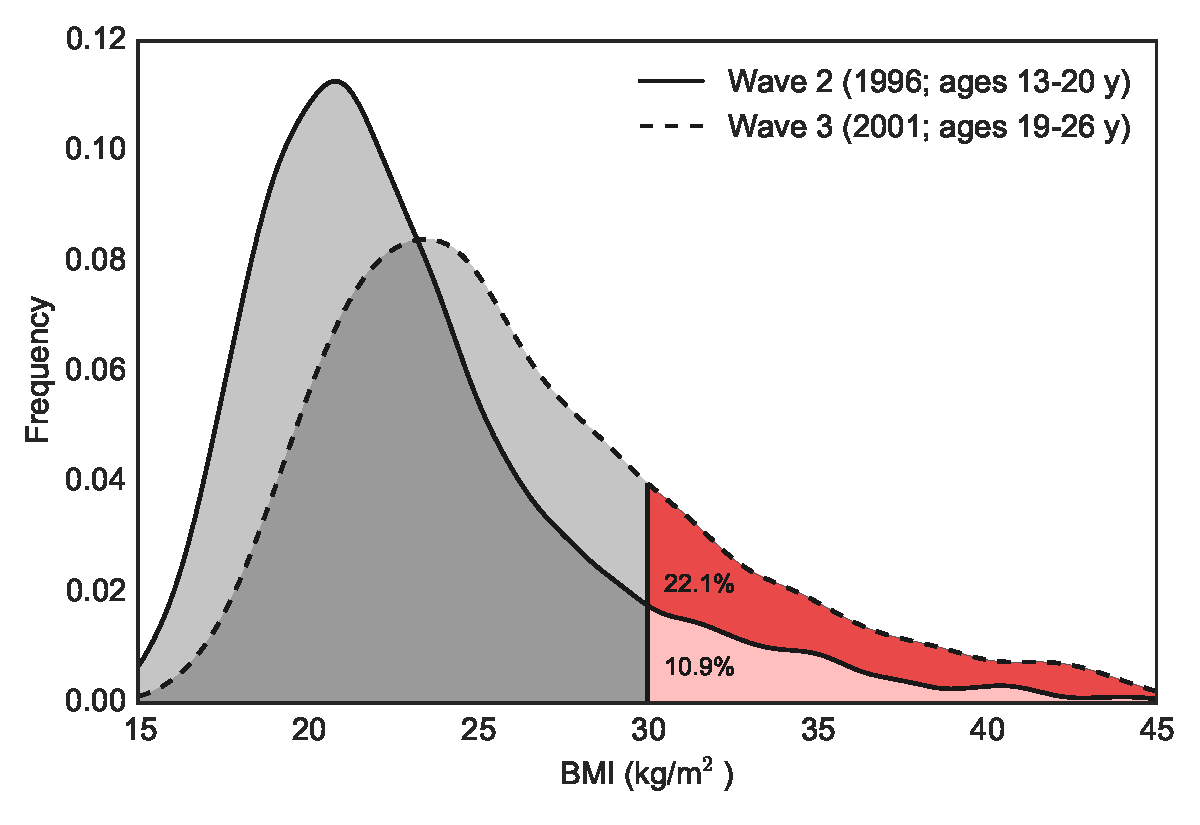
\includegraphics[width=1\textwidth]{plot.pdf}
\end{center}
\caption{Distribution frequency of BMI from the National Longitudinal Study of Adolescent Health (Add Health) waves II (1996; ages 13---20y) and III (2001; ages 19---26y). The transition between adolescence and young adulthood is a high risk period for weight gain. 10.9\% of young adults in wave II had a BMI $>30$ on the basis of adult cutoffs, a number which increased to 22.1\% in wave III.}
\end{figure}

\clearpage
\begin{lstlisting}
import numpy as np
import pandas as pd
import seaborn as sns
import matplotlib.pyplot as plt


cols2 = {'Gender': 'BIO_SEX2',
         'Age': 'CALCAGE2',
         'Weight': 'H2WS16W',
         'Height (ft)': 'H2WS16HF',
         'Height (in)': 'H2WS16HI'}

cols3 = {'Gender': 'BIO_SEX3',
         'Age': 'CALCAGE3',
         'Weight': 'H3WGT',
         'Height (ft)': 'H3HGT_F',
         'Height (in)': 'H3HGT_I'}


def calc_bmi(df, d=2):
    if d == 2:
        cols = cols2
    elif d == 3:
        cols = cols3

    df = df[list(cols.values())].convert_objects(convert_numeric=True)
    df['weight_lbs'] = df[cols['Weight']]
    df['height_in'] = df[cols['Height (in)']]
    df['height_in'] += 12 * df[cols['Height (ft)']]
    df['bmi'] = df.apply(lambda x: (x['weight_lbs']/x['height_in']**2) * 703, axis=1)
    df = df[1 < df.bmi]
    df = df[df.bmi < 100].dropna()

    return df

def load_data():
    df2 = pd.read_csv('Data_Wave02.tsv', sep='\t')
    df3 = pd.read_csv('Data_Wave03.tsv', sep='\t')

    df2 = calc_bmi(df2)
    df3 = calc_bmi(df3, d=3)
    return df2, df3

def plot(df2, df3):
    sns.set(style="white", color_codes=True)
    f, ax = sns.plt.subplots()
    sns.kdeplot(df2.bmi, ax=ax, shade=True, color='k', gridsize=10000, clip=(15, 45))
    sns.kdeplot(df3.bmi, ax=ax, shade=True, color='k', ls='dashed', gridsize=10000, clip=(15, 45))

    plt.legend(['Wave 2 (1996; ages 13-20 y)', 'Wave 3 (2001; ages 19-26 y)'], fontsize=15)
    plt.xlim(15, 45)

    ax.annotate('10.9%', xy=(25, .02), xytext=(30.5, .005), color='k')
    ax.annotate('22.1%', xy=(25, .04), xytext=(30.5, .02), color='k')

    y1 = ax.lines[0].get_ydata()
    x1 = ax.lines[0].get_xdata()
    x_mask1 = np.ma.masked_less_equal(x1, 30).mask
    y_masked1 = np.ma.masked_array(y1, x_mask1)

    y2 = ax.lines[1].get_ydata()
    x2 = ax.lines[1].get_xdata()
    x_mask2 = np.ma.masked_less_equal(x2, 30).mask
    y_masked2 = np.ma.masked_array(y2, x_mask2)

    ax.fill_between(x2, np.zeros_like(y2), y_masked2, facecolor='red', interpolate=True, alpha=0.5)
    ax.fill_between(x1, np.zeros_like(y1), y_masked1, facecolor='white', interpolate=True)
    ax.fill_between(x2, np.zeros_like(y2), y_masked2, facecolor='red', interpolate=True, alpha=0.25)

    plt.vlines(x=30, ymin=0, ymax=0.0398, color='k', linewidth=2, alpha=1)#, ls='dashed')

    plt.xticks(size=15)
    plt.yticks(size=15)

    plt.ylabel('Frequency', fontsize=15)
    plt.xlabel('BMI (kg/m$^2$)', fontsize=15)
    plt.tight_layout()
    plt.show()


if __name__ == "__main__":
    df2, df3 = load_data()
    plot(df2, df3)
\end{lstlisting}
% \lstinputlisting{plot.py}

\end{document}
